\graphicspath{{chapters/03/}}

\chapter{Genetic Fingerprinting}
Genetic fingerprinting is a tecnique used to identify some characteristics of a genome (a pattern of variable elements), like SNPs or minisatellites, in order to uniquely characterize a genome.\\
Genetic fingerprinting can be used to compare a genome with a reference sample or to compare different genomes between each other, in order to determine their diversity or analogy. 

DNA fingerprinting is applied in different fields:

\begin{itemize}
	\item In Forensic, for identification purposes;
	\item In lineage related tests, for cells or humans. Eg. pternity test, hereditary tests.
	\item For the certification of the origin of cells used in the laboratory, to make sure that the cells are the right ones and that there are no major geentic drifts. Needed when using certain cell lines, for publishing purposes.
\end{itemize}


\subsection{Variants used for genetic testing}

There are different variants that can be used for genetic fingerprinting, such as Single Nucleotide Polimorfisms (SNPs) or inherited Copy Number Variations (CNVs).
SNPs are substitutions of a single nucleotide at a specific position in the genome, whereas copy number variation is a phenomenon in which sections of the genome are repeated and the number of repeats in the genome varies between individuals.
Basically everything that is inherited and that is a polimorphism can be used in genetic testing, however some variants are more amanable than others.
SNPs are the most amenable ones since they are simple, abundant in the genome and easy to detect in sequencing data at any coverage depth. For these reasons, in this lesson we will focus on the development of SNP-based genetic tests.

\section{SNPs features}

\subsection{Hardy-Weinberg equilibrium and Minor Allele frequency}

One property of SNPs which has to be taken into account when using SNPs for genetic testing is the \textbf{Hardy-Weinberg equilibrium}. 
In population genetics, the Hardy-Weinberg equilibrium states that allele and genotype frequencies in a population will remain constant from generation to generation under neutral selection, so in the absence of other evolutionary influences, like genetic drift, mate choice, sexual selection, mutation and so on.

In the simplest case of a single locus with two alleles denoted \emph{A} and \emph{a} with frequencies f (A) = p and f (a) = q, respectively, the expected genotype frequencies under random mating are f (AA) = $p^{2}$ for the AA homozygotes, f (aa) = $q^{2}$ for the aa homozygotes, and f (Aa) = 2pq for the heterozygotes. In the absence of selection, allele frequencies p and q are constant between generations, so equilibrium is reached.
SNPs that respect this equilibrium are also the most studied, thus more informative. 

\subsection{Minor Allele Frequency}

Also, when performing genetic fingerprinting, the aim is to maximize the probability to have different genotypes in unrelated individuals. 
For this reason, the more advantageous SNPs will be the ones in which the allelic frequency of the variants is the higher possible. Highest variability in the population allows to distinguish better more individuals. 

Number-wise, a frequency of $\frac{1}{3}$ for each SNP would maximize the variability, but those SNPs wouldn't be in HW equilibrium and we might have missed calls. 
Therefore, the optimal SNPs to detect individuals’ differences and similarities are those with genotype frequencies: $P_{AA}$ = 0.25, $P_{BB}$ = 0.25, $P_{AB}$ = 0.5. 50\% of individuals for that SNP will have a heterozygus genotype, 25\% a homozygus genotype for the reference allele, 25\% for the alternative allel.

This is equivalent to say that best SNPs will be the ones with \textbf{MAF} = 0.5. Minor allele frequency (MAF) is the frequency at which the second most common allele occurs in a given population.

\bigskip
Some useful projects:
\begin{itemize}
	\item \textbf{dbSNPs}: is a database of small scale nucleotide variants. The database includes both common and rare singlebase nucleotide variation (SNV), short (=< 50bp) deletion/insertion polymorphisms, and other classes of small genetic variations.
	\url{https://www.ncbi.nlm.nih.gov/snp/}
	
	\item \textbf{HapMap3}: is teh third phase of the HapMap project whose aim is to develop a haplotype map of the human genome to describe the common patterns of human genetic variation in order to allows researchers to find genes and genetic variations that affect health, disease and individual responses to medications and environmental factors. The HapMap is a catalog of common genetic variants that occur in human beings. It describes what these variants are, where they occur in our DNA, and how they are distributed among people within populations and among populations in different parts of the world.
	\url{https://www.sanger.ac.uk/resources/downloads/human/hapmap3.html}
\end{itemize}

\subsection{Haplotype Blocks}

Another important feature to consider for SNPs selection are \textbf{Haplotype blocks}. Haplotype blocks are blocks along the genome that tend to be inherited as segments (no recombination inside a haplotype block). In these sizable regions there is little evidence for historical recombination and only a few common haplotypes are observed. \\

So for example, if there are 10 SNPs in a block of 1 MB, the genotype of one specific SNP in that block gives an indication the genotype of the other SNPs in the same block, since they are inherited together. 
Hence, if there is a haplotype block, there is no point in sequencing all SNPs in that block, it is sufficient to select some specific SNPs. Also, when running a fingerprint assay, there is no point in using all SNPs in a haplotype block since they won't bring additional information independently.\\

SNPs in the same HB are said to be in \textbf{Linkage Disequilibrium} (LD). Linkage disequilibrium measures the non-random associations between alleles or polymorphisms at different loci. A higher LD indicates a SNPs with a stronger tendency to co-segragate.
Haplotype Blocks are therefore commonly represented with \emph{linkage disequilibrium plots} \ref{fig:linkage}. In these plots, SNPs are represented in a way that does not respect the genomic distance, but the order along the genome (position of each SNP relative the others). 

% aggiungere LD plot - slide 7
\begin{figure}
	\centering
	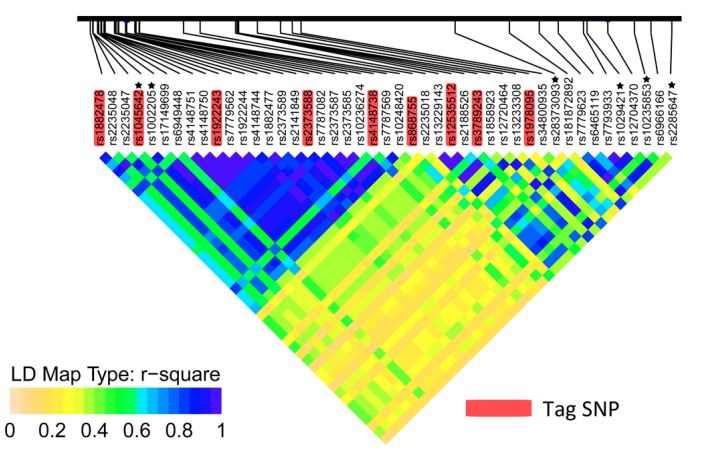
\includegraphics[width=0.7\textwidth]{linkage.png}
	\caption{\label{fig:linkage}LD plot of SNPs with top-ranked bayes factors in CHB (Han Chinese in Beijing) of 1000 Genome Phase I. The colors indicate the
strength of pairwise LD according to r2 metrics. The SNPs marked with asterisks represent independent strong associations. Tag SNPs are here shadowed in pink.}
\end{figure}

The colors indicate the strenght of pairwise linkage disequilibrium (LD) according to r2 metrics. In fact, not all of the SNPs are informative to distinguish between individuals. 
In \ref{fig:linkage} \textbf{Tag SNPs} are shadowed in pink. A Tag SNP is representative of a region with high linkage disequilibrium and represents a group of SNPs (called haplotype).


\subsection{Other SNPs features} 
\begin{itemize}
	\item Choose SNPs that are in areas that are not likely to undergo somatic aberrations. So exclude chromosomal locations which undergo frequent somatic aberrations. Eg. areas commonly deleted in tumor will produce LOH but probably also no calls, since there is no DNA. 
	\item Choose SNPs equally represented/spread all around the genome (not in specific chromosome regions).
	\item Select autosomal only SNPs (not on chromosome X).
	\item Select SNPs in exons. If we were to run a targeted assay, this would cover more exons instead of intrones. It will also be more probable to have signal from a non-DNA assay, for example if calling a genotype from RNA sequencing data (even though it is not always done).
	\item Exclude/include disease or drug response associated loci. 
	\item Include/exclude loci with significantly different MAF in different ethnicity. If we include them we can also have a lineage type of tests in the same assay. 
\end{itemize}


\subsection{Number of SNPs to select} 

If we want to build a test to run genetic fingerprinting using SNPs, \textbf{how many polymorphic loci (SNPs) should be tested?} 
We want to make sure that the measure of the test will be able to differentiate unrelated individuals. 
But we must also remember that many variables must be taken into account, possible mismatches in particular. Those can be due to the sequencing process itself (experimental mismatches) but also to changes due to somatic events (biological mismatches). All these events can be used in the test with a different weight, based on how likely they are. 


\subsubsection{Experimental mismatches : Genotype call error rate}

During sequencing, each machine will produce some errors, resulting in some loci for which no data will be available. If those loci include some SNPs of interest, then no call will be associated to that SNP. 
Experimental mismatches are related to the error rate of the technology used, they are platform dependent. 

\paragraph*{Some examples:}

\begin{figure}
	\centering
	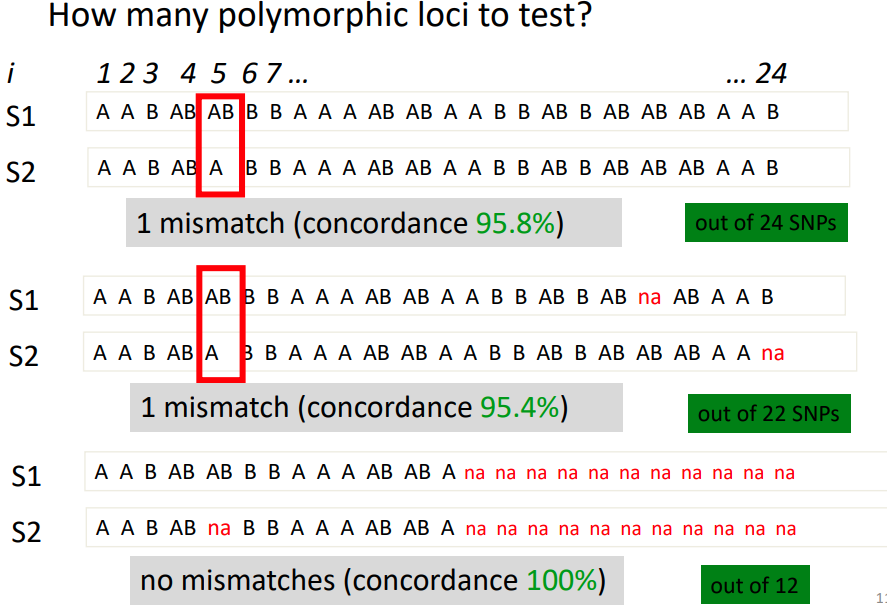
\includegraphics[width=0.7\textwidth]{SNP.PNG}
	\caption{\label{fig:SNP}}
\end{figure}

In each example in figure \ref{fig:SNP} there are two samples with the same number of potential SNPs: 24. To detemine the difference/similarity of the two samples we can look at the genotype for each position and count mismatches.

Legend: 
'A' stands for 'AA' (e.g. homozygus genotype for the reference allele); often refered to as Aa.
'B' stands for 'BB' (e.g. homozygus genotype for the alternative allele); often refered to as Bb.
'AB' stads for heterozygus.

\begin{itemize}
	\item First Example: over the 24 loci, there is only one mismatch. This translates to a level of concordance of 95.8\%. Those 2 individuals are highly related or DNA comes from the same saples.    
	\item Second example: there is only one mismatch but there are some 'na', indicating that for some positions we don't have a call (not available data). Therefore, in this case the concordance is measured out of 22 SNPs and is equal 95.4\%. 
	\item Third example: here a lot of nas are present, leading to have only 12 SNPs available. This brings to a concordance of 100\%. 
\end{itemize}

Different examples produced different levels of concordance. What do we trust the most?

The first set of SNPs is the one that we trust the most, because it has the higher number of available SNPs. Wider number of SNPs provides the most reliable information. 

\subsubsection*{Biological mismatches}

In the context of desease samples and tumors, many somatic events can happen, like deletions, gains of copies, homozygus deletions, ecc. Some common ones are:
\begin{itemize}
	\item  Loss Of Heterozygosity (LOH):  event that results in loss one parental copy of a region which results in the genome having just one copy of that region. If that region contained a heterozygus locus (e.g. SNP), there will be loss of Heterozygosity.  
	
	AB -> A.
	\item Gain Of Heterozygosity (GOH): due to a mutation in a site often polimorphic through inheritance. These are pretty rare.
	A -> AB. 
	\item Double Mutation (DM): very rare.  
\end{itemize}

\bigskip
Biological mismatches can be properly modeled in our assay. We can, in a data driven way, assess the error rate for the genotyping for some specific SNPs or run tests. We can also think in terms of SNP-specific or tissue-specific probabilities.

The main point is that all mismatches must be taken into consideration. 
For this, all implemented tests use \emph{more than the minimal number of SNPs} that allow to identify individuals. 


\section*{Genetic Distance}

Having defined the number of SNPs to use, with maximum MAF and other amanable characteristics, the genetic test should provide a measure of some sort, which will be the output metric, associated with a probability of the measure to be correct. 

As a simple measure, we can count the number of loci where two samples show different genotype and normalize on the total number of queried loci, defining a certain level of discordance (or concordance). The output value will be the 'genetic distance' between the two samples given the selected loci. The distance is proportional to the number of discordant calls.

In figure \ref{fig:Distance} we can see an example of a typical graph used to measure the genetic distance using SNP-based genetic testing. We have 4 samples with a set of 5 SNPs for each one. The distance is measured among all possible pairs, whose indexes are reported on the x-axis. 
\begin{itemize}
	\item s1 and s2 have 3 A in common, one locus has no call and another one produces a mismatch. 1 mismatch out of 4 produce a distance of 0.25.
	\item samples s1 and s2 have 5 mismatches out of 5, so a distance (or discordance) of 1. 
\end{itemize}

% figura
\begin{figure}
	\centering
	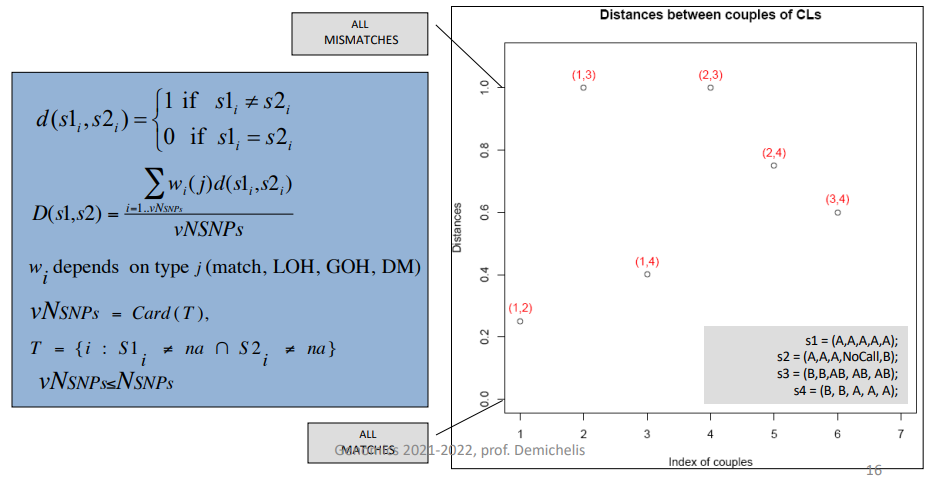
\includegraphics[width=0.7\textwidth]{loci.PNG}
	\caption{\label{fig:Distance}Genetic Distance graph with 4 samples}
\end{figure}

If we put that into an equation will have that: for each position i (SNP) bwteeen sample 1 and 2 we can have 1 if the genotype is different, 0 if they are identical. Then we determine the distance D by summing up the different scores obtained for each SNP. We can associate different weights $w_i$ to different mismatches or we can put all equal to one. Then we devide by the total number of SNPs for which we have available calls, vNSNPs, which will be lower or equal to the total number of SNPs, NSNPs. 

%
\begin{figure}
	\centering
	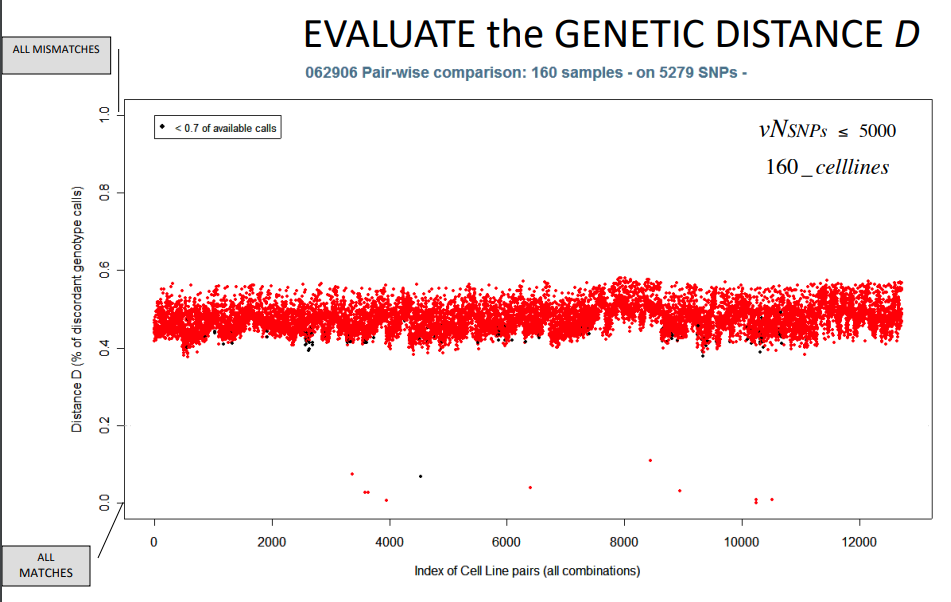
\includegraphics[width=0.7\textwidth]{loci2.PNG}
	\caption{\label{fig:Distance2}Genetic Distance graph with 160 samples}
\end{figure}

\bigskip
This other example at figure \ref{fig:Distance2} shows the distance, measured by genetic fingerprinting, of a collection of 160 samples of cell lines. 

The number of possible pairs corresponds to: 160 * 159 / 2 (number found in the x-axis). 

By applying this measure to a larger collection of samples like this one, with many SNPs, we expect to find an \textbf{average distance} among all possible pairs that very unlikely will be close to 1. 
The MAF of the SNPs is 0.5 but it will never happen that, with a high number of SNPs, the discordance will be 1. We will have an average distance that in this case around 0.5, since by chance we all share some genotypes on a large number of SNPs. 

Here they found certain pairs with a very low distance, sometimes almost equal to zero (dots at the bottom). This was a surprising result because it shows that those pairs, which were suppose to be different cell lines, were actually not different cell lines (only less than 70\% of SNPs have available calls). 

% immagine slide 19
\begin{figure}
	\centering
	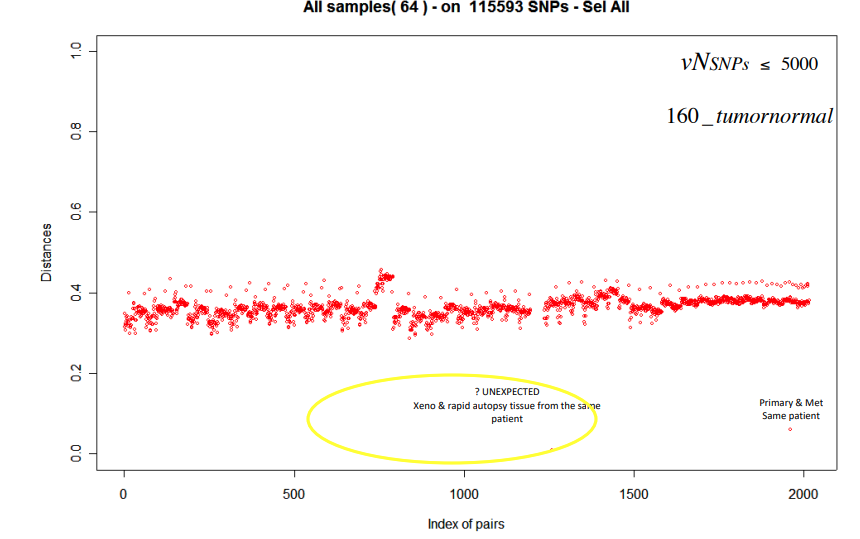
\includegraphics[width=0.7\textwidth]{loci3.PNG}
	\caption{\label{fig:Distance3}Genetic Distance graph with tumor samples}
\end{figure}

\bigskip
In this last example at figure \ref{fig:Distance3} genetic fingerprint was performed on a collection of 160  tumor samples, with a larger SNP array (more that 100.000 SNPs).  

From the analysis, two samples with very low distance were observed. One of the two samples came from a 
Rapid Autopsy Progam and the other one from a xenograft model. 

RAP are programs for which patients at the end of their life agree to donate their tumor tissues which can be used for research. In these very complex but highly valuable programs, the material must be taken within two hours after death. Those sample are usually higly caractherized but after a while the track of the patient's identity is lost. 
Here, what happened is that one man who donated tissue by this program was sequenced and for some of those metastasis models were generated and implanted into a mouse and a xenograft model was derived. Thanks to fingerprinting it was possible to determine the same origin between xenograft and patient. 

The power of this tecnique is very high, it allows also to identify and remove things that we don't want in our study. Eg. if running a study (like a GWAS study) on a certain interesting geopraphic area, we will want to remove the members of the same family because that would skew the results. Genetic fingerprint can be used for this purpose.

\subsection{Some questions}

\textbf{Q1}: Would the average of unrelated samples distance increase or decrease after selection of ideal SNPs?

If we maximize the likelihood that SNPs have a different genotype among individuals and we use these to determine the measure, then the average distance of unrelated individuals will increase.

\textbf{Q2}: Is it likely to obtain a genotype distance D = 1?

We get distance 1 only if we are looking at too few viable SNPs. Whereas with a well selected pool of SNPs, and a high enough number of SNPs, it is very unlikely that the distance is equal to 1.

\subsection{Further considerations}
How does the genetic distance among different samples change when varying the number of selected SNPs used to perform the test?

% immagine slide 26
\begin{figure}
	\centering
	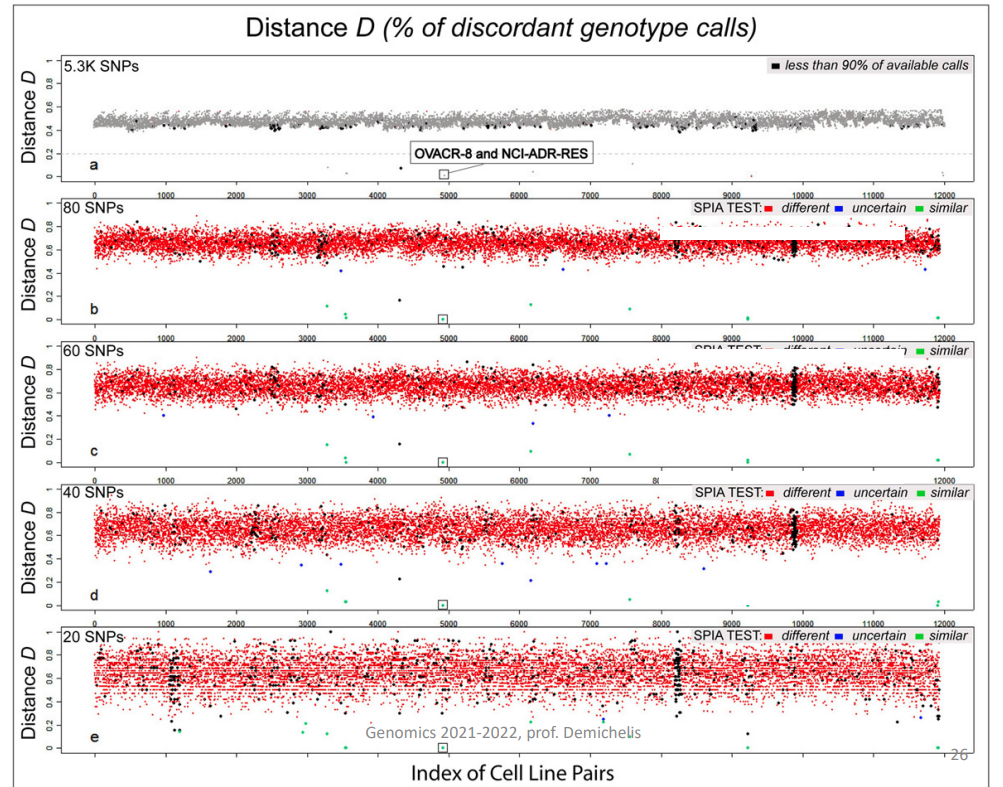
\includegraphics[width=0.7\textwidth]{selected.PNG}
	\caption{\label{fig:sel_snp}Genetic Distance graph at deacreasing number of selected SNPs}
\end{figure}

The genetic distance among many samples, with an array of 5.3K SNPs, was measured, using a decreasing number of SNPs (from the initial total number of SNPs to decreasing numbers of highly selected SNPs) \ref{fig:sel_snp}. 

It is noticeable that, in the second plot where 80 SNPs matching the required characteristics were selected, the average Distance across all pairs is higher than in the previous example, in which all available SNPs were used (~0.45 vs. ~0.65). Also, the standard deviation of greater. 
Decreasing the number of SNPs to 60, then to 40 and 20 leads to have the same average distance between pairs, which settles around 0.66, but higher standard deviation.

In reality we always need enough SNPs, enough information, in order to prevent unexpected issues and to be sure that for any pairs of sample we have enough information to trust our measure. 


\section{Building a SNP-based genetic test}

Building an identity test base on SNPs is a MULTI-STEP process, consisting in: 
\begin{enumerate}
	\item Definition of a genotype/genetic distance to compare samples;
	\item Definition of SNPs requirments, based on the intention of the assay.
	\item Selection of SNPs:
	\begin{itemize}
		\item This can be done in a data-driven manner, through an iterative procedure of training and test on known sample set;
		\item Or, performing the selection based upon MAF and Hardy-Weinberg equilibrium. For example, using HapMap data.
	\end{itemize}
	\item Implementation of a probabilistic test (different, uncertain or similar)
	\item In silico validation on independent/multiple dataset.
	\item Validation on cell lines genotyped on independent platform. 
\end{enumerate}
We have already seen some of the steps needed (1, 2, 3), we now pass to the following ones.


\subsection{Implementation of a probabilistic test} 

Other important questions which we have to answer to when designing a genetic test are:
\begin{itemize}
	\item What is the threshold on the genotype distance to call two samples 'identical' ('similar') or'different'?
	\item How confident would the call be?
    \item What is the minimum number of loci needed for a robust test?
\end{itemize}

It could be useful to have a probabilistic test to determine if the measure of the test is correct at with which level of confidence. We can use a probabilistic approach to compare observations with expectations (gold standard).

\bigskip
Under the assumption that SNP calls at different loci are independent, we can think in terms of Binomial distribution. Each SNP can be considered as a trial, n = number of SNPs in the assay, k = number of matches, p is the probability of match and (1-p) of mismatch. Then the probability of having k matches (successes) out of N SNPs (trials) follows the binomial distribution.

With n, np and np(1-p) large enough, we can use the Gaussian approximation of the Binomial distribution with $K_{mean}$ = np and sd = np(1-p). 

With somtehing that simple we can add a probabilistic test in our assay, defining an area of conficence given by $K_{mean} \pm m * sd$ where m is the number of standard deviations used to define the thresholds which will lead to have a smaller or wider confidence area. 

%immagine slide 33
\begin{figure}
	\centering
	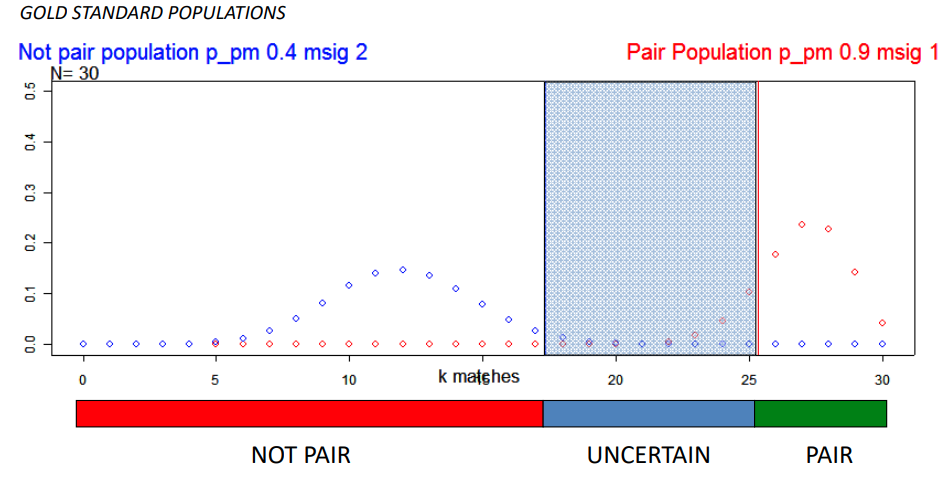
\includegraphics[width=0.7\textwidth]{double_test.PNG}
	\caption{\label{fig:prob_test}}
\end{figure}

\bigskip
So for example: given two unrelated samples, we reason in terms of 'what is the probability of having a certain number k of matches over a total number of n SNPs, therefore a certain value of D?'. 

The probability mass function for unrelated individuals is shown in figure \ref{fig:prob_test} with a blue dotted line and indicates that there is a low probability of having both a very low and a very high number of matches. 

We can also think in the opposite term: given two related samples, what is the probability of having  matches? As represented by the red dotted line, in this case there will be a high probability of having many matches. 

Using these probabilities we can set two thresholds which will define 3 regions:
\begin{itemize}
	\item A \textbf{'not pair'} region for which the two samples will be considered as 'different'
 	\item a \textbf{'pair'} region for which the two samples will be considered as 'similar'
	\item and an \textbf{'uncertain'} region, a grey zone, for which no certain result can be produced. 
\end{itemize}

Then we can move the grey area based on what we want to be certain of and on how many SNPs we have.

By decreasing the number of SNPs, the grey zone will become more tiny, making the result more difficult to interpret. For example, a difference of only 2 matches could lead to opposite conclusions. 

By contrast, with more SNPs the area will be wider and easier to interpret. Hence using a number of SNPs greater than the minimum number is better, otherwise there will be many uncertain calls. 


\section*{Further considerations and examples}
%sistemare
In the past, before sequencing area and SNPs array area, short tandem repeats were commonly used for genetic fingerprint. They were used on gels to distinguish related and unrelated individuals, eg, for the initial paternity test. 

\textbf{Inherited copy number variants} can be used too for a fingerprinting test, but not all of them. The more amenable for this test are the loss type of CNV. In the population there will either a copy number of 2 or 1 or 0. If both parents have heterozygus pair of CNVs it will be possible that I have a homozygus deletion. If both parents have 2 copies at a site that is polimorphic in the population, we will have a genotype equal to 2 copies. 

If we think about gain of CNV then it becomes messy, because when combining multiple copies and have a add up we cannot distinguish what comes from what pair, so we cannot use them to identify an individual.


\subsection{Example 1: Cell line passages}

A mass use of these genetic tests is done to assess genetic changes in in-vitro cultivation (also, in studies in tumor evolution, lineage plasticity, etherogenity across metastasis across individuals or a single tumor).
Cell lines go through multiple passages in which they are used and stored. Genetic fingerprinting can be used to assess if among different passages the cells have remained the same, if they were mislabeled or if major genetic drifts happened.

In this example, two types of prostate cell lines which underwent multiple passagges were used: N15C6 (passages from 48 to 63) and N33B2 (passages from 21 to 39).
The cell lines were profiled with a SNPs array and the assay was run.
All passages of each cell lines were compared with all other passages. We expect all passages to have the same genetic fingerprinting in the same cell line.  

However the results obtained using the full array of SNPs (50k), showed that some pairs which should be exactly identical (distance equal to zero) are actually a bit different (points at the bottom-left).
By contrast, by using a set on only 54 SNPs, this diversity is not detectable, indicating  that using the perfect number of SNPs could make us loose some information. 

% immagine slide 39 e 40
% con width = 0.4 le mette affiancate 
\begin{figure}
	\centering
	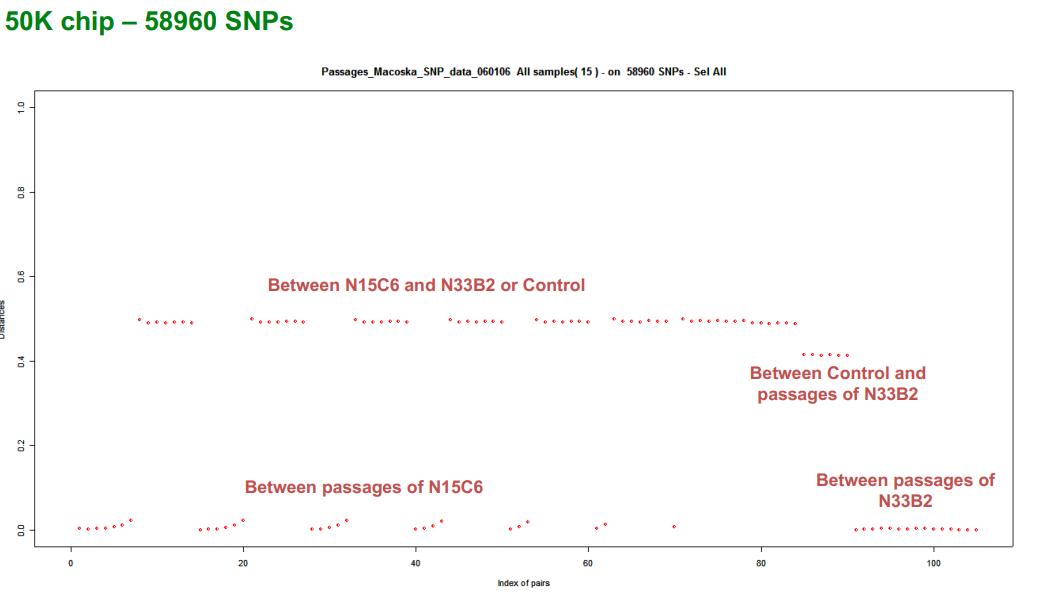
\includegraphics[width=0.5\textwidth]{50k.png}\quad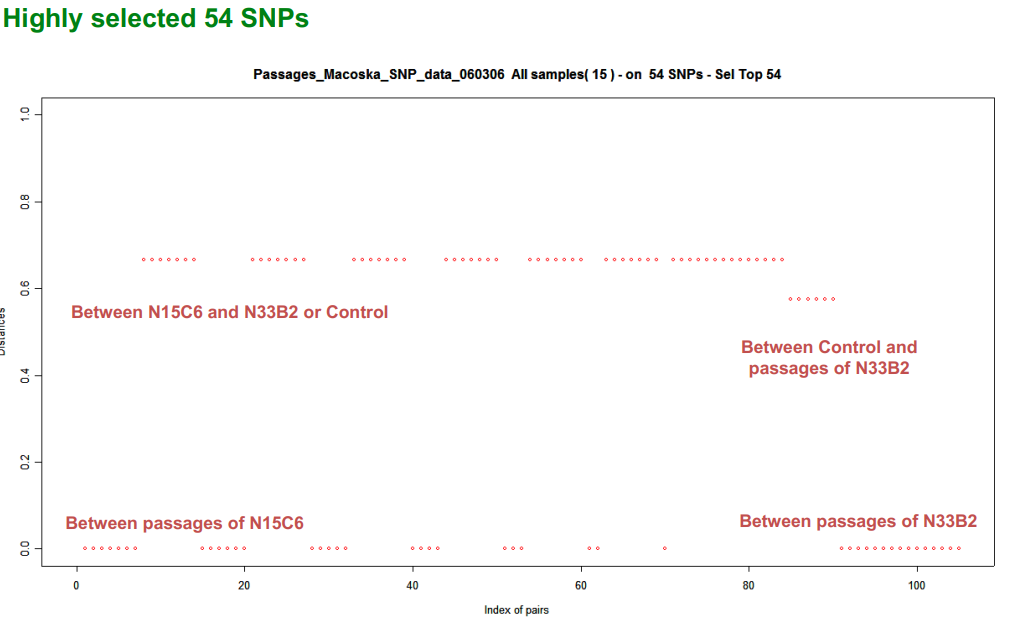
\includegraphics[width=0.5\textwidth]{54_snps.PNG}
	\caption{\label{fig: cell_lines}}
\end{figure}

In order to understand this increase of distance, they looked at each chromosome to see if there were problems that justified increase the increased distance expected to be equal to zero in that cell line. All chromosome were tried. If we focus only on the SNPs spread across Chromosome 11, we observe that there is a major difference for certain passages with respect to the initial ones, only for one cell line (N15C6). This was due to the way the cells were immortalized (insertion in chromosome 11).


\subsection{Individual's Relatedness (genotype-distance)}

The HapMap consortium sequenced hundreds of individuals for different ethnicities and also used trios. Trio sequencing is a technique which involves the sequencing of the genome of mother, father and son/daughter. Trios provide major information for haplotype blocks, for identifying regions related to inheritance, ecc. 

% immagine slide 43
\begin{figure}
	\centering
	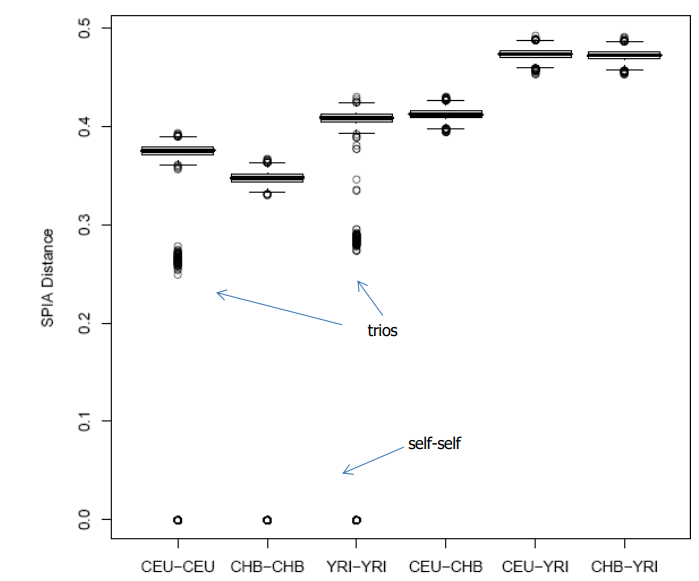
\includegraphics[width = 0.7\textwidth]{relatedness.PNG}
	\caption{\label{fig: trios}}
\end{figure}

By looking at the data based on SPIA Assay (a genotype base assay which measures distance) at figure \ref*{fig: trios} we see that self-self pairs have distance zero, as expected; samples within each ethnicity have a certain average distance, which is lower that the distance observed among different ethnicities. Differences in distance among mixed samples are due to the fact that the SNPs used had on average higher MAF in some populations than in others. We also notice that in trios the distance is not 0 and is not equal to the median distance of unrelated individuals. This can be used for paternity tests or even in forensic science.

\subsection{Example 3: Cancer supscettibility test}
The data showed refers to a study were they were looking for polimorphisms that increase the likelihood of prostate cancer. In these studies, if relatives are present in the cohort, only one of them is taken to avoid skewing the results. 
When looking for signs of cancer susceptibility by performing genetic fingerprinting, the division based on the degree of relativeness was determined 'for free' and could be used to remove unwanted samples from the cohort.


\subsection{Genetic structure of the human population}

One relevant aspect of the human genome is that it contains everything needed to learn about the genetic structure of the human population. 

Undestanding the geentic structure of human populations is of fundamental interest to medial, forensic and anthropological sceinces. 

Some of the reasons as to why knowing the genetic substructure of data is important:
\begin{itemize}
	\item The goal of association studies is to identify DNA variants that affect disease risk or other traits of interest. However, association studies can be confounded by differences in ancestry.
	\item Misleading results could arise if individuals selected as sidease cases have different ancestry, on average, than healthy controls. If in a study all controls are of the same ethnicity and the test is done on an individual of a different ethnicity than the test is biased.
 	\item If we run a GWAS study using two ethnicities and we want to uset the same markers of sucettibility worldwide, it won't work. 
\end{itemize}

Especially in medicine and in the study of human evolution it is important to track the genetic background of individuals that are involved in studies in order to understand if the individuals are form a homogeneous population or from genetically distant ones. 
More and more, clinical studies must have declarations of the checks and interpretation of the data of the genetic background of the individuals present in the study. It is very important to come to results for which we know exactly what is the applicability. To avoid spurious results, association studies often restrict their focus to a single continental group. 

Advances in high-throughput genotyping technology have improved the understanding of global patterns of human genetic variation and suggest the potential to use large sample sets to uncover variation among closely spaced populations.
One important piece of information to consider when developing methods to understand the genetic structure of a population, is to think in term of variance, which is also relevant for human diseases. 
Many SNPs have different MAFs in different populations. If we use those, and are able to have all of them in a simple computational way, we could be able to infer what is one individual's genetic background in terms of origins (e.g. chinese origins). 

The easiest mathematical approach to assess how well SNPs can distinguish ethnicity is by using \textbf{Principal Component Analysis (PCA)}. By running a very simple PCA on a set of SNPs including SNPs with different MAF in different populations we can, in a space, distinguish different ethnical groups. And we could also start thinking at individuals' origins. 

How accuratley can one predict an individuals geographic-ethnical background based upon his/her geentic barcode?

% study seen in the slides
\subsubsection{Example paper: 'Genes mirror geography within Europe'}

In the \href{https://www.ncbi.nlm.nih.gov/pmc/articles/PMC2735096/}{study seen during lectures} they used a 500.000 (500k) single nucleotide polymorphism array. Information about the country of origin of grandparents, parents and other relatives was used to determine the geographical location that best represents each individual ancestry. 
They run a combined study where they used a supervised search to find the best SNPs to make inference and then they tested it on another set of individuals. 
By using high confidence data (individuals with high confidence origin data) and by using the genotypes of highly informative SNPs for specific region-related inheritance, they were able to rebuild the map of some of the countries in Europe \ref*{fig:PCA_countries}. 

% immagine paper 
\begin{figure}
	\centering
	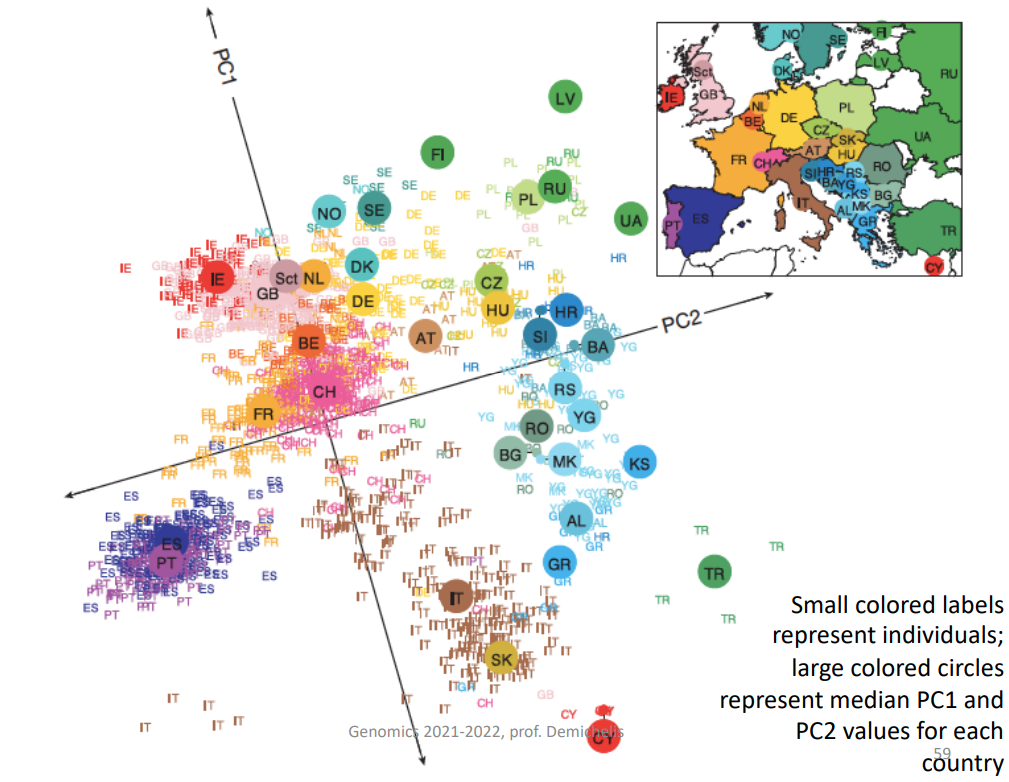
\includegraphics[width=0.7\textwidth]{population.PNG}
	\caption{\label{fig:PCA_countries}}
\end{figure}

This result might be a little bit of a push, but it is true that by using properly selected variants it is possible to distinguish individuals coming from different countries. The way those SNPs are selected is very similar to the process saw for genetic fingerprint, but pushing for the selection of variants that are different in terms of MAF in different populations. 

Clusters that are a bit more dense and distant from the others (like the Spain/Portugal cluster) could be due to the fact that many SNPs selected are typical of that area and are therefore able to maximize the difference with respect to that area (so it is a data-related 'issue').

% immagine 
\begin{figure}
	\centering
	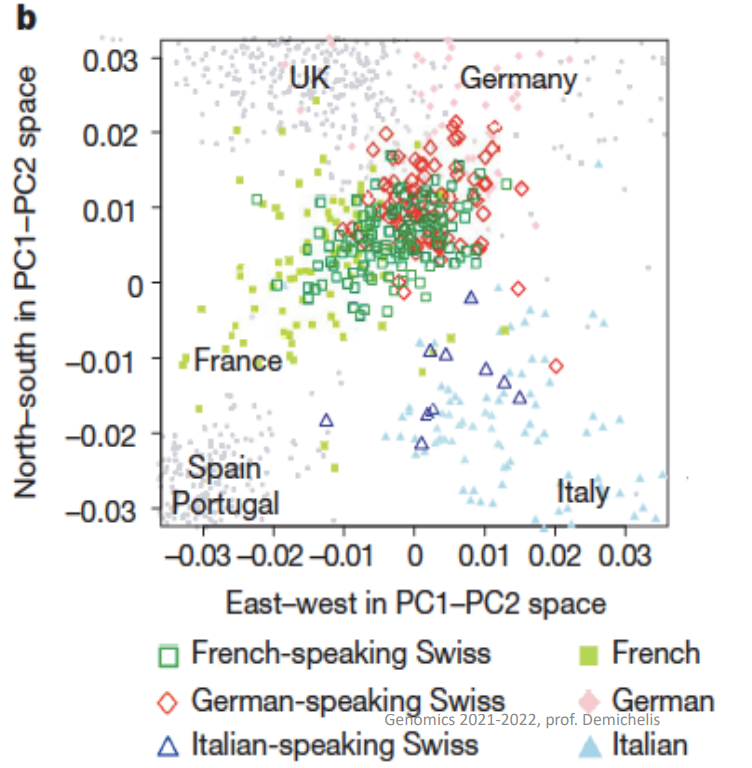
\includegraphics[width=0.7\textwidth]{swiss.PNG}
	\caption{\label{fig: PCA_swiss}}
\end{figure}

Focusing on Switzerland, they could even make inference on the linguistic canton \ref*{fig: PCA_swiss}. Again this is a bit of a push, but it is possibly true that in country where some regions have very different habits (e.g. marriage within the same area) might lead to have similar genetic fingerprint. 


\subsubsection{Summary and notes}
Low-frequency alleles tend to be the result of a recent mutation and are expected to geographically cluster around the location at which the mutation first arose. Hence, they can be highly informative about the fine-scale population structure.

Despite low average levels of genetic differentiation among Europeans, close correspondence between genetic and geographic distances was
found. When mapping the genetic basis of a disease phenotype, spurious
associations can arise if genetic structure is not properly accounted for.

